The idea behind atomic bonded crosschain debt is inspired by flash swaps. In a flash swap, the loan in not paid to the borrower unless she pays it back immediately at the same block as borrowed \cite{flashswaps}. In ABCD, this is extended to several blocks \ie  the bond can be payed back in more than one block but it contains a secret and the lender's signature in everywhere it is being used. 

Unsecured bonds or debentures are bonds that are not backed by some type of collateral. The concept of unsecured bond is so close to the late deposition swaption explained earlier. Since our bond is unsecured, the owner does not have to deposit any margin. Moreover, we need a margin free swaption to be used in further contracts. Hence, we have extended our \MetaSwaption model with a new stage named Delay Keeper to make new component achieving the desired goal.

% Unsecured bonds or debentures are bonds that are not backed by some type of collateral. In other words, .

\begin{figure*}
    \centering
    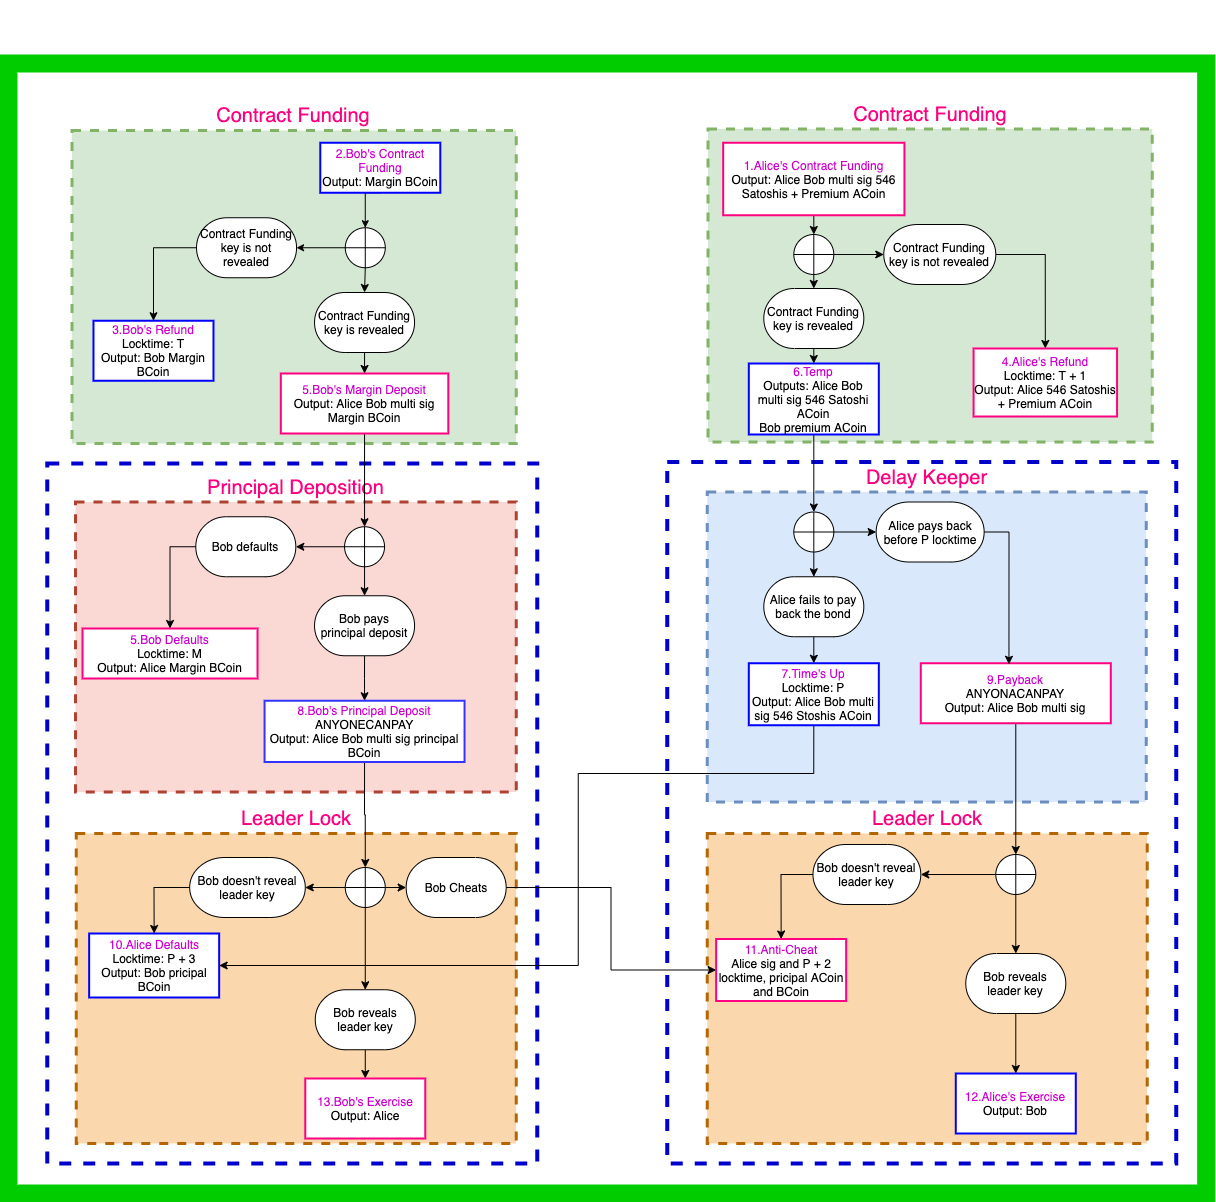
\includegraphics[width=\textwidth]{figures/non-collateralized-bond-no-checkseq.png}
    \caption{The Atomic Bonded Crosschain Debt component. Pink-bordered transactions are broadcast by Alice and blue-bordered ones by Bob.}
    \label{fig:non-collat-bond-no-checkseq}
\end{figure*}

\begin{itemize}
    \item \textbf{Contract Funding}: This stage is similar to swaption's Contract Funding stages. with slight changes in Alice's Funding:
    \begin{itemize}
        \item She does not deposit any margin.
        \item She deposits a very tiny amount for further usage\footnote{In the time we are writing this paper, minimum amount of output in Bitcoin network to be mined by miners is 546 Satoshis}.
    \end{itemize}
    
    \item \textbf{Principal Deposition}: Like the similar stages in swaption components, Bob is supposed to deposit his principal before M locktime.
    
    \item \textbf{Delay Keeper}: At this stage, Alice only has P locktime ($P > M$) to deposit her payback transaction. If she does not deposit, Bob will broadcast the {\it Time's Up} transaction that prevents Alice from fulfilling her Payback transaction. The {\it Temp} transaction is necessary so that we can have an HTLC to restrict Alice's payback deadline. 
    
    \item \textbf{Leader Lock}: If Bob has fulfilled his principal, Alice has P locktime to payback Bob's money. The procedure of this stage is: 
    \begin{itemize}
        \item Alice succeeds to payback Bob's bond. Then Bob reveals the \keyone key The bond is given to Alice and paid back to Bob.
        \item Alice fails to pay back till P, so Bob avoids exposing the \keyone key and his get his principal back.
        \item Alice fulfills her payback transaction but Bob avoids revealing the \keyone key.Now Alice can broadcast the Anti-Cheat transaction which sends her principal and an amount of punishment from Bob's principal to her. 
    \end{itemize}

    Note that if Bob delays in broadcasting the {\it Time's Up} transaction, Alice may broadcast the {\it Payback} and {\it Anti-Cheat} transaction at the very last minute and cheat on Bob.

\end{itemize}

Since Alice's {\it time's Up} transaction needs to be shared in both Alice's and Bob's stages, this form of bond can not be used in different blockchains. To solve the problem of interoperability for our atomic bond we have redesigned our model by using CHECKSEQVERIFY which is explained in \Apn{\ref{app:non-collat-bond}} 